%!TEX root = ../MasterThesis.tex

\chapter{Conclusion and Future Work} % (fold)
\label{cha:conclusion}

\section{Conclusion}
\label{sec:conclusion}

Initially, this Master thesis started with three fundamental assumptions: \@

\begin{enumerate}
	\item the use of an unsecure computer network to transfer credit card information in the \gls{E-commerce} scenario make them always subject to frauds and counterfeits,
	\item the existing technological solutions to detect and prevent them will not be able to cover 100\% due to the complexity and dynamics of the whole system, and
	\item the substantial analysis of any suspicious transaction is not taken place today due to the enormous effort and time needed to collect all required information manually
\end{enumerate}

As this Master thesis has pointed out in Chapter~\ref{cha:introduction} and Chapter~\ref{cha:context_analysis} the first and second premise has been seen a lot of research and development in recent years. But neither an industry-wide usage of the \gls{PCI/DSS} standards to securely process personal and payment-related information, nor the widely adoption of rule-based or score-based fraud prevention systems has been able to stop deceivers from cheating the \gls{E-commerce} system and bringing harm to the merchants and consumers alike. Whereas the Master thesis has shown the impact of \gls{E-commerce} frauds to the merchants, who are usually the ones that have to cover the losses, it also makes clear that any successful fraud attempt will reduce the thrust into the \gls{E-commerce} system, which is a substantial part of the global economics already. \\

Thus, bringing down the amount of fraudulent transactions in the system cannot be done with technology alone, but require a sharing of information between experts coming from various organizations. As the Master thesis explained in Section~\ref{subsec:e_commerce_fraud_handling} this consolidation of information about a suspicious transaction is currently not being done in-depth as this would require a lengthy manual communication and analyzation process by the investigator of an issuer or \gls{PSP}. This fact has lead to the third premise as well as to the hypothesis that the introduction of a collaborative system, which makes use of Semantic Web and peer-to-peer communication technologies to collect the information and know-how of the relevant stakeholders and link them together, can improve this siutation significantly. \\

As explained in Section~\ref{sec:system_approaches} existing approaches for integrating information from different sources are either to restrictive to work on a large scale (Web services), or are to open for the sharing of personal and payment-related information (Semantic Web). Therefore a new proposal for a collaborative system has been developed in Chapter~\ref{cha:system_concept} and Chapter~\ref{cha:system_design}, which uses suitable aspects from the Semantic Web standards as well as a secure \gls{P2P} communication network between the stakeholders for collaborating on \gls{E-commerce} fraud incidents. \\

Due to the fact that the information will be provided from dispersed organizations the proposed solution have to deal with differences in structure and wording of them. In these circumstances the \gls{W3C} standards such as \gls{RDF}, \gls{RDFS}, \gls{OWL} and \gls{SPARQL} show their full potential. As part of the Semantic Web initiative they already solve these issues on a global scale. Still, those standards only provide the basics for integrating distributed information. Additional steps are required to build intelligent applications on top of them. In Chapter~\ref{cha:system_concept} the Master thesis showed that the information has to be combined into a graph-oriented representation of the \gls{E-commerce} activities done with a credit card recently. Based on the initial clustering of order details by merchant a subsequent mapping and linking of the information has to be done to be able to cluster the transactions on different aspects with the objective to find abnormal activities. \\

As Chapter~\ref{cha:system_design} showed the Semantic Web standards provide various axioms in the \gls{RDFS} and \gls{OWL} specifications to support the mapping of information using different schemata. Based on these statements the \gls{RDF} data store (especially the reasoner in it) can \emph{infer} additional attributes (aka relations) into the combined data set. These mapping expressions can be either managed and injected by the participant doing the merging of the information from different sources, or can be integral part of the shared data sets already. Particularly the latter option will ease the integration of different data sources, but requires the participants to look into commonly used \gls{RDF} vocabularies or ontologies. A selection of the available vocabularies that might fit the \gls{E-commerce} fraud investigation was also depicted in this Chapter. In addition to the mapping of the information certain aspects of them have to be linked together to be able to cluster and analyze them in detail. Linking information on the Semantic Web relies on either using the same unique \gls{URI} for the identical objects in different data sets, or infer equality based on property constraints set in the schema definitions. An explanation of those options can also be found in Chapter~\ref{cha:system_design}. \\

At the end the proposed solution was using a partially centralized \gls{P2P} architecture that has the issuer of a credit card at its center. This decision was taken as the issuers are the stakeholders, who will figure out about suspicious activities on a credit card in the scenario selected for this Master thesis. They will have to decide whether a transaction is fraudulent or not. In those edge cases, in which the fraud prevention system is unsure about the status of a transaction, an investigator of the issuer will initiate a collaborative session with affected participants. Those parties will share their relevant information with the issuer and collaborate on the investigation of the cases. Due to the fact that the issuer as a financial institution has to follow strict regulations and data protection laws, there should be no serious problems for sharing detailed order information with them. Still, some of the information of the stakeholders might be critical and have to be obfuscated somehow. Available methods to do that are part of the partially centralized system design of this Master thesis. \\

Thus, this Master thesis have shown that the technical issues that lead to fraudulent transactions in the \gls{E-commerce} scenario could not be solved completely by introducing new security procedures, but require a collaboration of different experts on the case. This collaboration can become more efficient and effective if a shared information space is used that combine and link together the information from the relevant stakeholders. The existing Semantic Web and \gls{P2P} communication technologies can act as enabler to design and develop such as collaborative system.

\section{Towards a decentralized \gls{P2P} system}
\label{sec:p2p_decentralized_system}

In the decentralized P2P system architecture each node is equal and keeps their local data ready for analysis if the node is online. If the issuer will have to figure out, whether a transaction is fraudulent or not, she is going to send out various queries to all the available nodes in the P2P cluster asking for certain information that help investigating the case. The other nodes, whose reside on each stakeholder involved, will answering the queries based on the common Schema.org data mapping shown above and send back the results to the issuer bank. The issuer will collect all the results from the various parties and combine them to be able to analyze the issue and come up with a conclusion. The main benefit of this architecture is, that there is no need to duplicate the data from the other stakeholders to the issuer. Due to this it can also be a better suited solution if data sharing faces restrictions due to law or regulations. On the other hand this architecture will depend on the nodes being online all the time so the issuer can query for information at any time. So this works only in synchronous communication mode. Additionally there are efforts spread around all the stakeholders to set up and maintain a system for secure data querying functionality, please see Figure~\ref{fig:images_p2p_decentralized}.

\begin{figure}[H]
	\centering
		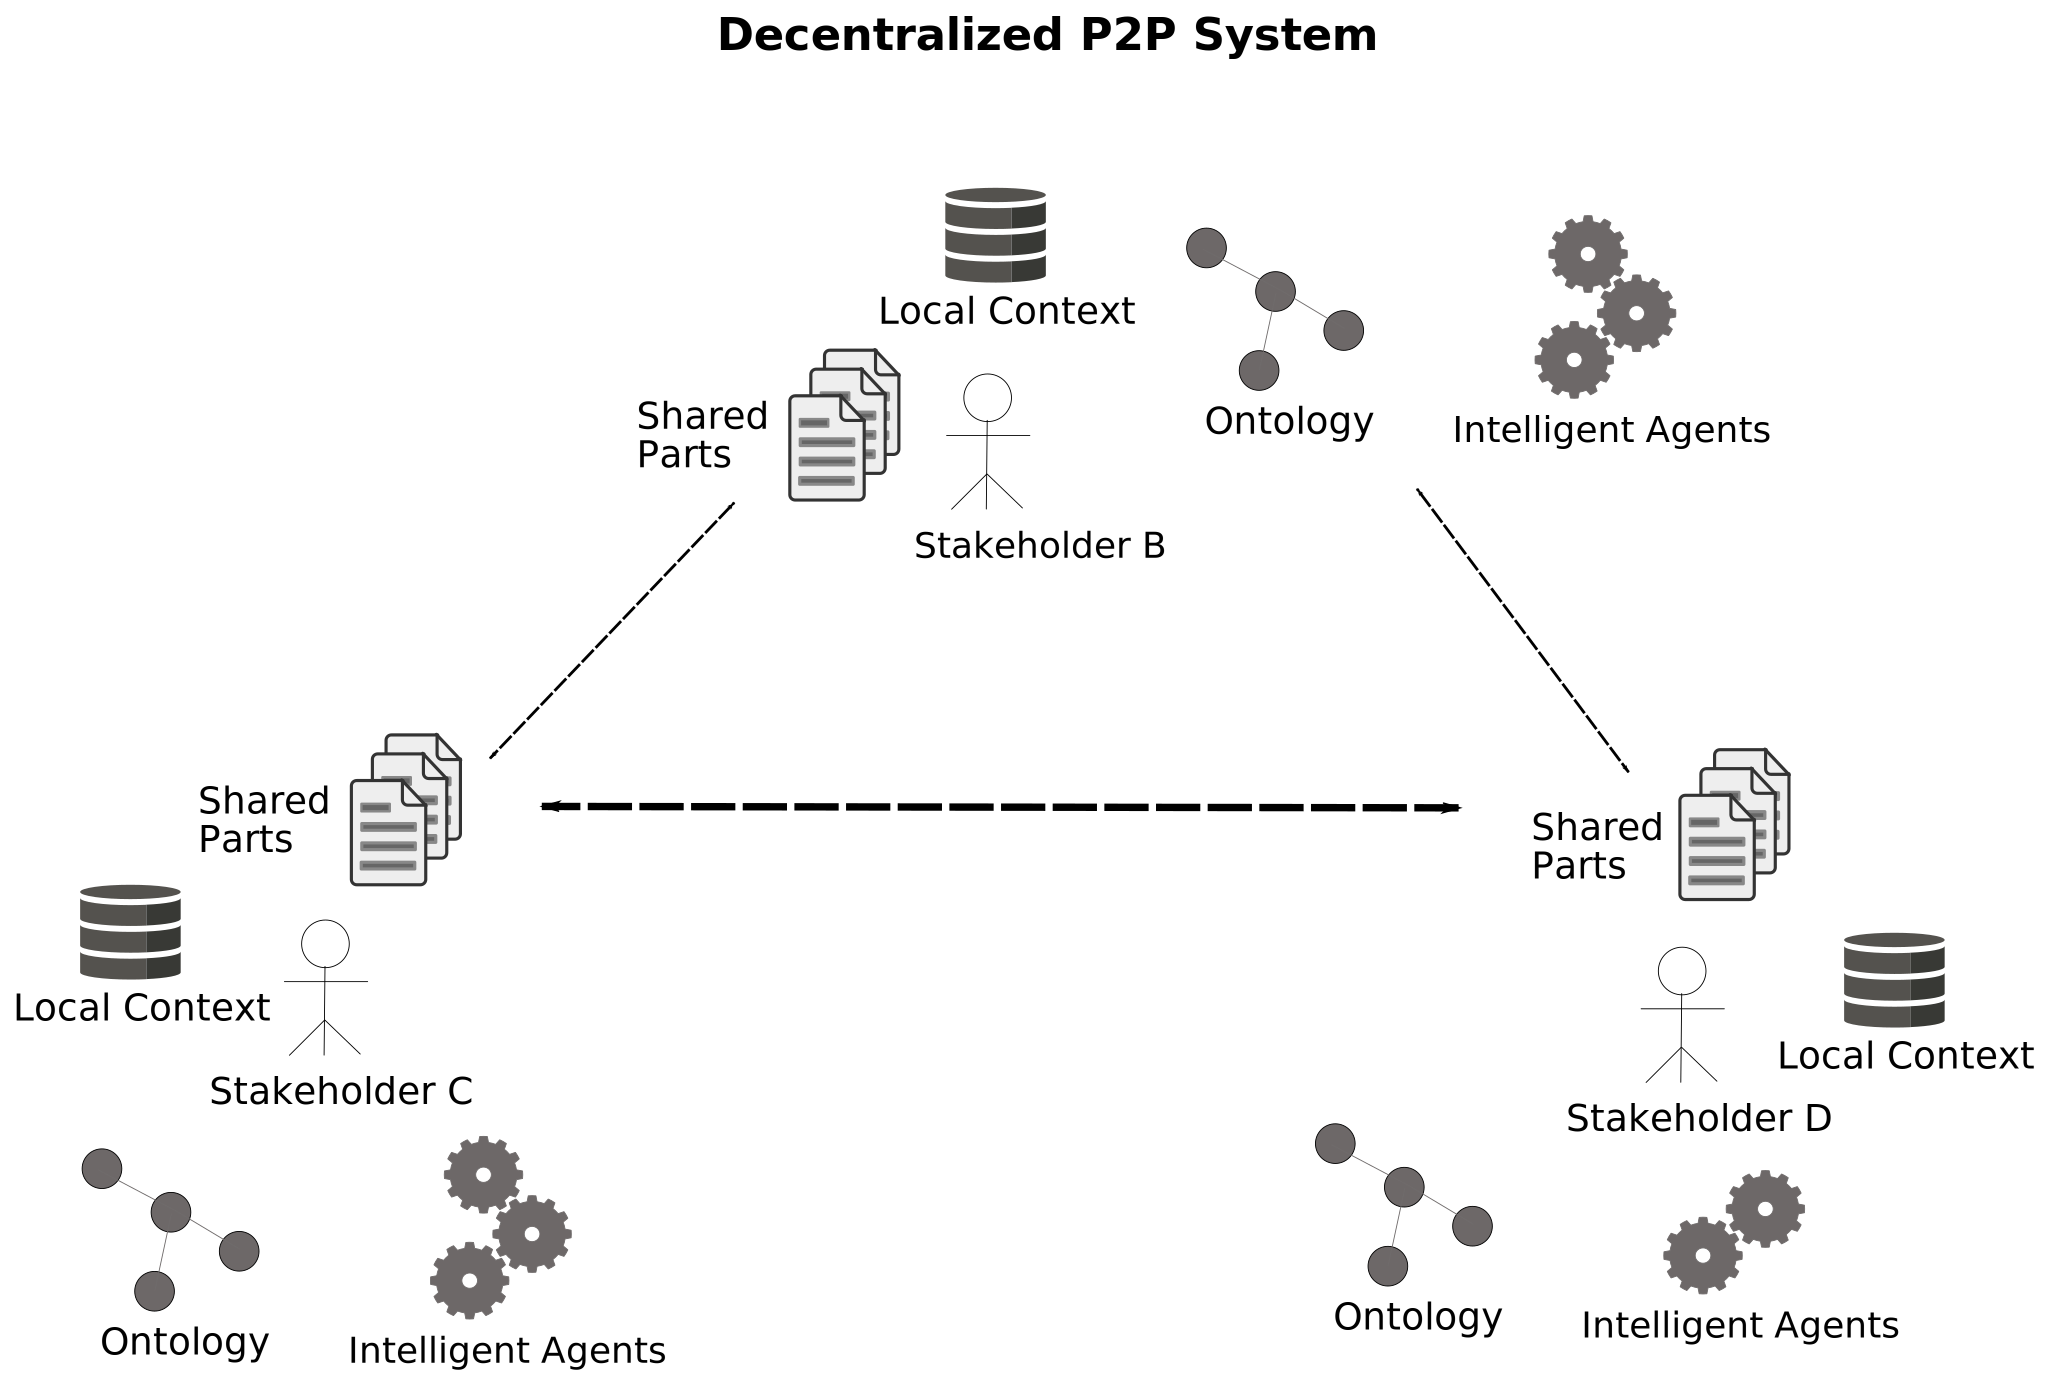
\includegraphics[width=0.9\columnwidth]{images/system_P2P_decentralized.pdf}
	\caption{Decentralized \gls{P2P} system architecture}
\label{fig:images_p2p_decentralized}
\end{figure}

% sec p2p_decentralized_system

% chapter conclusion (end)
